\documentclass{../source/Experiment}

\major{信息工程}
\name{}
\title{FM 信号的发送和接收实验}
\stuid{}
\college{信息与电子工程学院}
\date{\today}
\lab{——}
\course{通信原理实验}
\instructor{金向东、龚淑君}
\grades{}
\expname{FM 信号的发送和接收实验}
\exptype{仿真+验证}
\partner{}
\begin{document}
\makecover
\makeheader
\section{FM 接收实验}
在这个实验中,我们使用 USRP 设备做 FM 收音机收听 FM 广播。实验步骤如下:

(1)打开 GNURadio Companion 软件

(2)新建一个流程图页面,将 Options 属性的 ID 改为 LAB1,将 Variable 的 Value 改为 250e3。 Options 块定义该 grc 流图的属性。ID 为标题,也决定了生成的 py 文件的文件名。生成选项 Generate Options 可以选择 QTGUI/WXGUI/NoGUI,对应使用的 GUI 库的类型。在这里选择某 个 GUI 库后,在流图中的 GUI 模块就只能使用该库中的模块。

(3)添加 UHD USRP Source 到画布上。

(4)添加两个 QT GUI Range 模块,并将其属性改为如下所示。QTGUIRange 模块是一个可在 运行时调整的变量,ID 是变量名。程序运行时将会出现一个滑动条,滑动游标或者直接设 置数值可以在运行时实时改变变量值。

(5)添加一个 QT GUI Sink 模块,用于观测接收信号的信息。

(6)添加一个 Rational Resampler 模块,用于采样率变换。Rational Resampler 模块的 Interpolation 属性为差值倍数。其插值倍数为 audio\_rate*audio\_interp。

(7)添加一个 Variable 模块,其 ID 设置为 audio\_interp,其 Value 值设置为 4。

(8)添加一个 Variable 模块,其 ID 设置为 audio\_rate,其 Value 值设置为 48000。

(9)添加一个 WBFM Receive 模块,用来实现 FM 接收。

(10)添加一个 Audio Sink 模块,用来输出声音。将其 Sample Rate 设置为 audio\_rate。

(11)流图连接好后,保存为 LAB1.grc。

\begin{figure}[H]
    \centering
    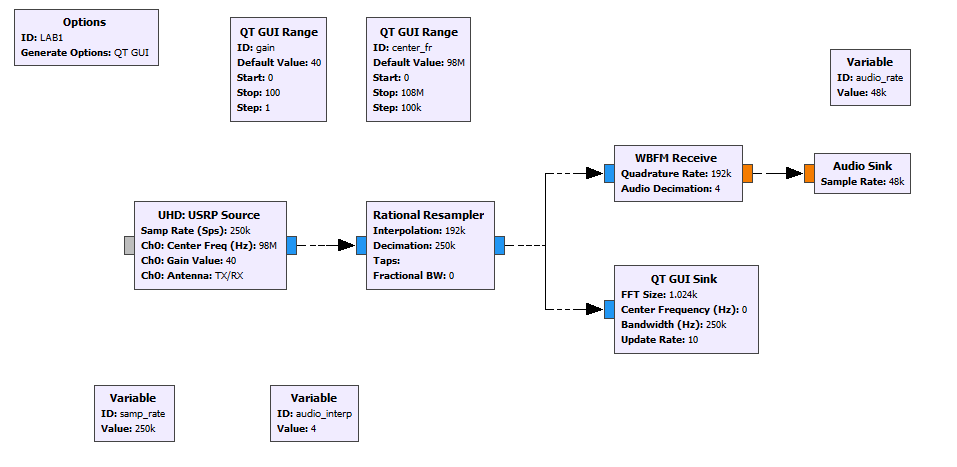
\includegraphics[width = 0.9\textwidth]{lab7/receive.png}
    \caption{接收实验}
\end{figure}

(12)将 USRP-B210 设备连接到 PC 端,然后运行程序。通过调节 center\_fr 的值来调节频道, 接收 FM 信号。

\begin{figure}[H]
    \centering
    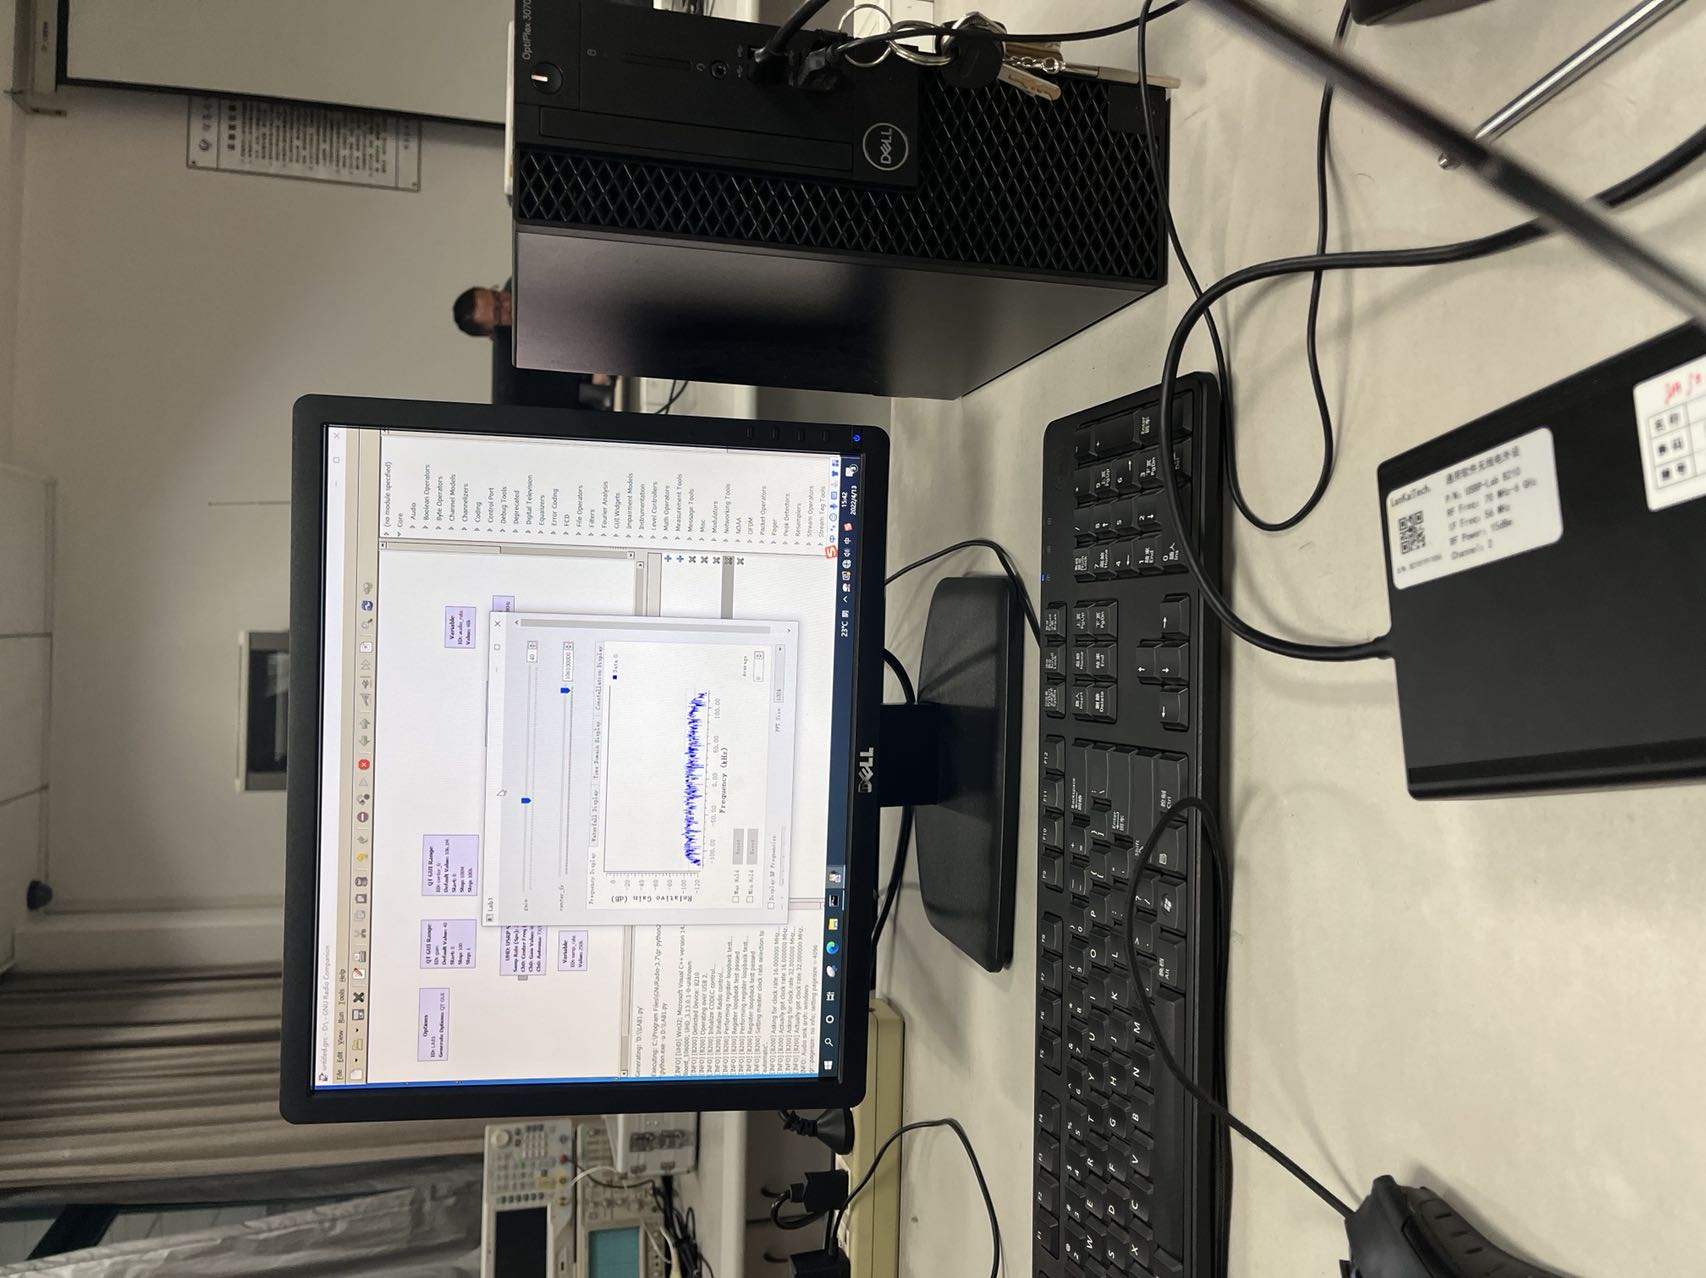
\includegraphics[width = 0.5\textwidth,angle=270]{lab7/1.jpg}
    \caption{流图结果1}
\end{figure}

\begin{figure}[H]
    \centering
    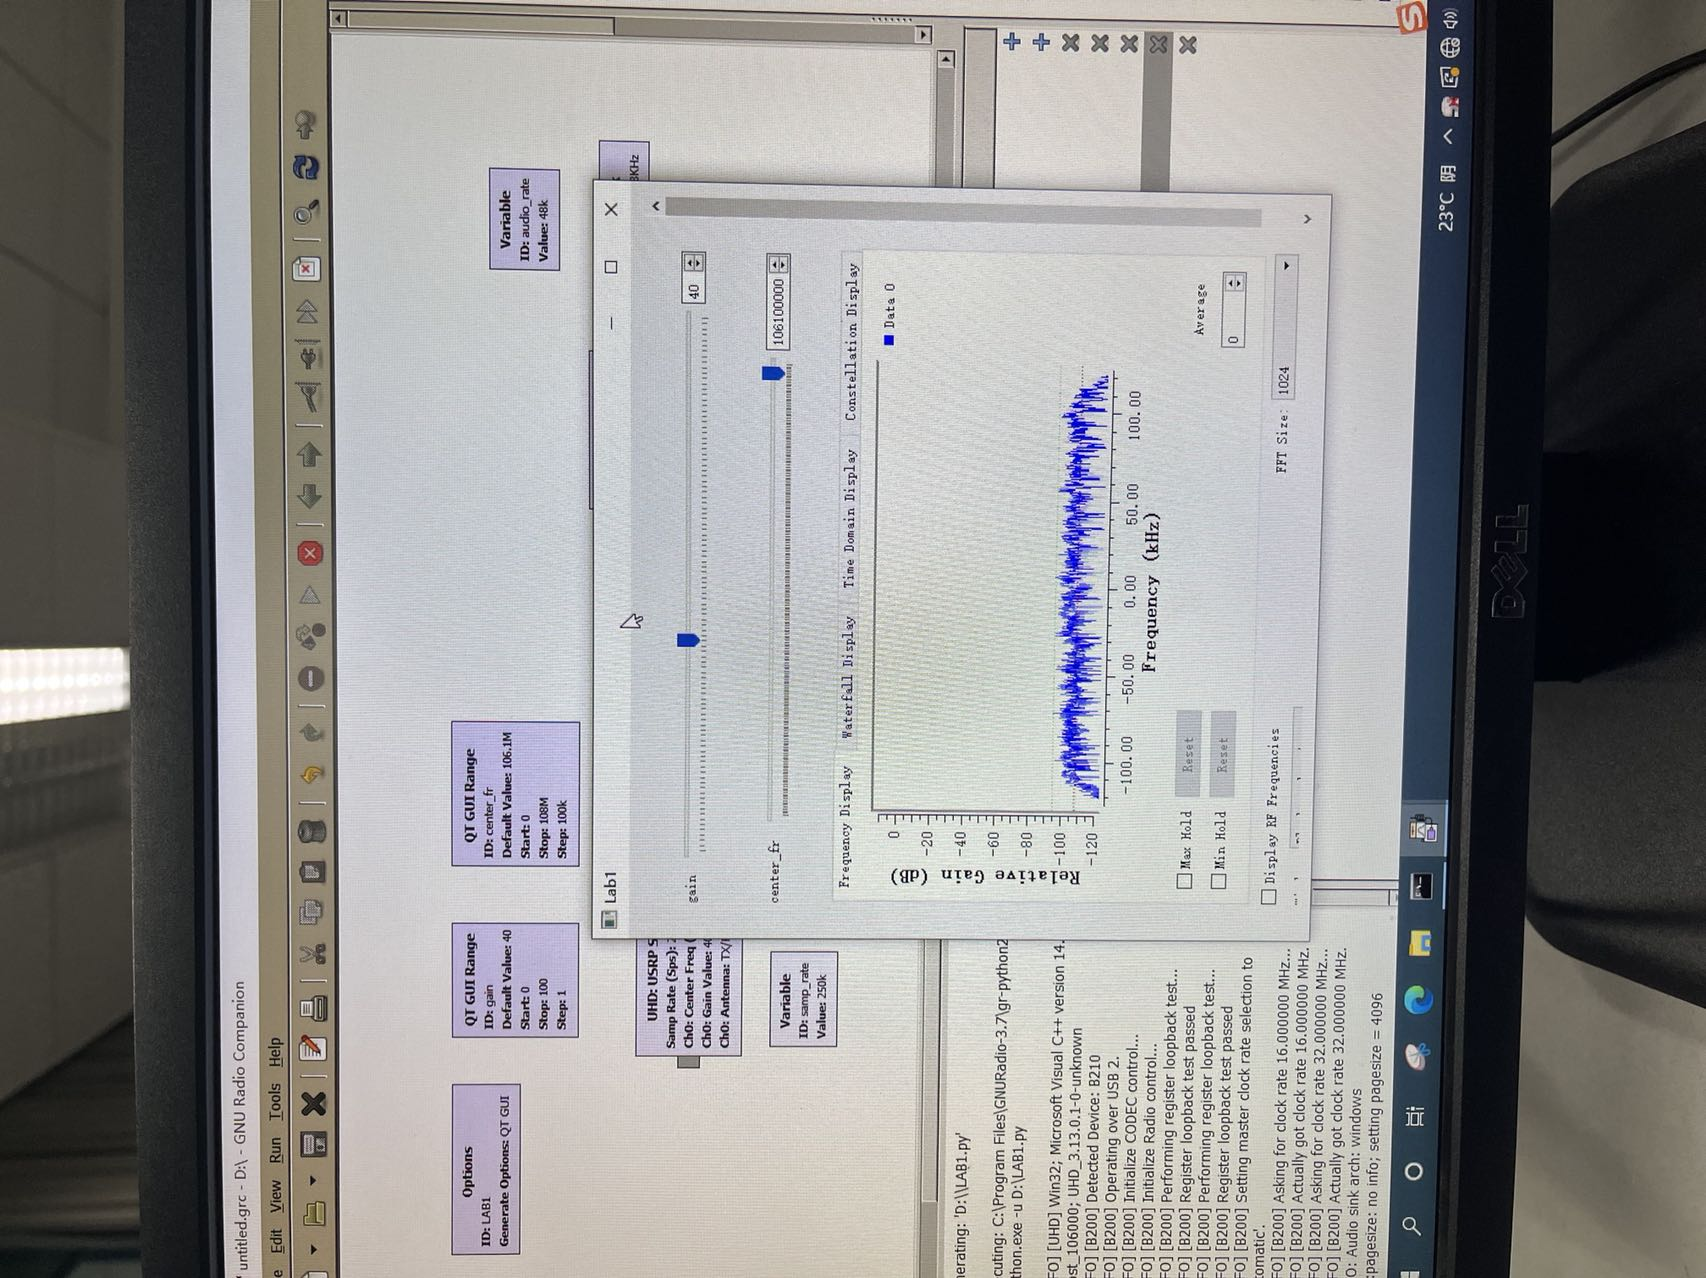
\includegraphics[width = 0.5\textwidth,angle=270]{lab7/2.jpg}
    \caption{流图结果2}
\end{figure}
\section{FM 发送实验}
先搭建好 FM 发射信号流图,然后用搭建的 FM 发射机发 送音频信号,在普通 FM 收音机中收听到音乐,并且用另一台 SDR 硬件接收,通过 FM 接收 机流图在计算机上听到音乐。

\begin{figure}[H]
    \centering
    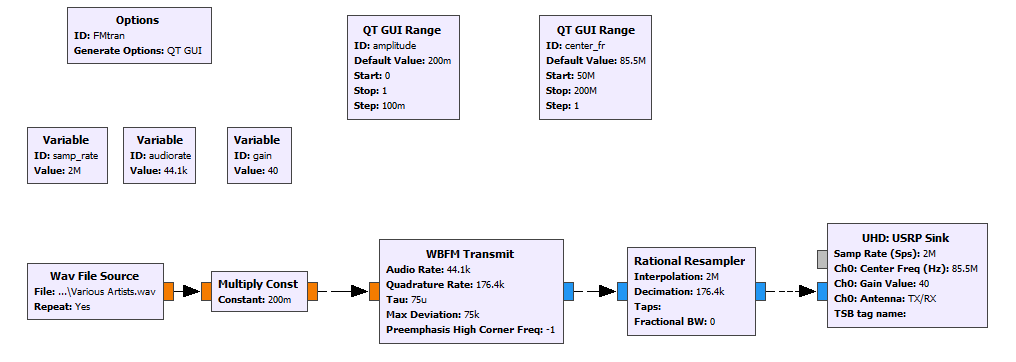
\includegraphics[width = 0.9\textwidth]{lab7/send.png}
    \caption{发送实验}
\end{figure}

一个完整的 grc 流图需要至少一个信源和信宿。这里的信源采用 wav 文件,该模块会将 声音内容转换为信号流(如 wav 文件的采样率为 44.1kHz)。信宿 UHD:USRP Sink 为 USRP 硬 件接口,可以设置中心频率和增益。设置的中心频率即为 FM 广播的频段,可以自由调整。

FM 调制方式通过 WBFM Transmit 模块实现。该模块共有 5 个参数:Audio Rate 表示音 频输入流的采样速率;Quadrature Rate 表示输出流的采样速率,与 Audio Rate 之间呈整数倍 关系;Tau 代表 pre-emphasis time constant,即预加重时间常数;Max Deviation 代表最大频 偏;Pre-emphasis High Corner Freq 代表预加重拐角频率,当该参数小于 0 时,默认值被设置
为 0.925*quad\_rate/2.0。

通过 WBFM Transmit 模块后,数据的采样速率为 176.4kHz,通过 Rational Resampler 重 采样模块调整采样速率至 2MHz。

流图绘制完毕后,如果流图符合要求,GRC 界面上的运行按钮就会处于可用状态。连接 HackRF,单击运行按钮,流图就开始运行。此时可以用收音机收听广播了。

在这个实验中我们组电脑中的wav文件出了问题无法成功发送,所以我们组从网上找了另外的歌曲文件,并转换成44.1kHz在8.71MHz频率处发射出去,旁边小组的同学用上一实验中的程序接收到,实验成功。
\end{document}